\documentclass[spanish]{beamer}
% ---------------------------------------------------------------
% Versión revisada. Cambios principales respecto al original:
%  * UTF-8; se eliminan paquetes sin uso (geometry, dsfont, cancel, amsfonts).
%  * Logo mediante \graphicspath (no hay rutas absolutas dentro del texto).
%  * Correcciones: \mathbf faltante, l -> L/\mu en Binet, "latus" -> semilado recto,
%    overlay <3- >, signo/módulo de f(r), g = -grad(phi) explícito, angulo alpha
%    en el flujo (theta queda reservado para el ángulo polar), volumen \mathcal V.
%  * Pasos intermedios faltantes (du/dtheta, dV/dr) y derivación de e(E,L).
%  * Nuevas diapositivas: punto de partida, teorema de la cáscara, problema
%    inverso resuelto, clasificación de órbitas, verificaciones, actividad IA,
%    extensión computacional, resumen.
% ---------------------------------------------------------------
\usepackage[utf8]{inputenc}
\usepackage[T1]{fontenc}
\usepackage{lmodern}
\usepackage[spanish]{babel}
\usepackage{amsmath,amssymb,mathtools}
\usepackage{booktabs}
\usepackage{graphicx}
\usetheme{Madrid}
\usecolortheme{beaver}
\usepackage{textpos}

% Figuras locales y logo institucional (ajustar si cambia la carpeta)
\graphicspath{{Figuras/}{/Users/luisnunez/Dropbox/MisDocumentos/UIS/UISImagenInstitucional/}}
\addtobeamertemplate{frametitle}{}{%
\begin{textblock*}{15mm}(.88\textwidth,-1cm)
\includegraphics[height=0.4in,keepaspectratio]{UISLOGO.png}
\end{textblock*}}

% Notación
\newcommand{\vr}{\mathbf r}
\newcommand{\ur}{\hat{\mathbf r}}
\newcommand{\Vef}{V_{\mathrm{ef}}}

\title{\textbf{El problema de Kepler y la ecuación de Binet}}
\author[L.A. Núñez]{\textbf{Luis A. Núñez}}
\institute[UIS]{\textit{Escuela de Física, Facultad de Ciencias,} \\
\textit{Universidad Industrial de Santander, Santander, Colombia} \\
{\includegraphics[height=0.4in,keepaspectratio]{UISLOGO.png}}}
\date{\today}

\begin{document}
\maketitle

\begin{frame}{Agenda}
  \tableofcontents
\end{frame}

%==================================================================
\begin{frame}{Objetivos de la sesión}
Al finalizar, el estudiante podrá:
\begin{enumerate}
\item Derivar la ecuación diferencial de la órbita (Binet) a partir de la ecuación radial.
\item Resolver el problema directo para $V=-k/r$ y expresar $e$ y $q$ en función de $E$ y $L$.
\item Usar la ecuación de Binet para resolver un problema inverso.
\item Clasificar las órbitas keplerianas combinando la solución exacta con el potencial efectivo.
\item Justificar, mediante la ley de Gauss, el modelo de masas puntuales y reconocer sus límites.
\end{enumerate}
\end{frame}

%==================================================================
\begin{frame}{Punto de partida: lo que ya sabemos}
\begin{itemize}
\item<1-> Dos cuerpos $\Rightarrow$ un cuerpo equivalente: $\vr=\vr_2-\vr_1$, masa reducida
$\mu=\dfrac{m_1m_2}{m_1+m_2}$, potencial central $V(r)$.
\item<2-> Simetrías y cantidades conservadas (Noether):
  \begin{itemize}
  \item isotropía $\Rightarrow$ $\mathbf L$ constante: movimiento plano, $\theta$ cíclica, $L=\mu r^2\dot\theta$;
  \item homogeneidad del tiempo $\Rightarrow$ $E=\tfrac12\mu\dot r^2+\Vef(r)$, \ $\Vef=V+\dfrac{L^2}{2\mu r^2}$.
  \end{itemize}
\item<3-> Ecuación radial:
\[ \mu\ddot r-\frac{L^2}{\mu r^3}=-\frac{dV}{dr}. \]
\item<4-> Hoy: especializar a $V=-k/r$ y obtener la \alert{forma geométrica de la órbita} $r(\theta)$ sin resolver primero $r(t)$.
\end{itemize}
\end{frame}

%==================================================================
\section{Gravitación: campo, ley de Gauss y modelo puntual}
\begin{frame}{El campo gravitacional}
\begin{itemize}
\item<1-> Sea $\vr=\vr_2-\vr_1$ la posición de $m_2$ respecto de $m_1$; $r=|\vr|$, $\ur=\vr/r$.
\item<2-> Energía potencial y fuerza que $m_1$ ejerce sobre $m_2$:
\[ V(r)=-\frac{Gm_1m_2}{r},\qquad \mathbf F=-\nabla V=f(r)\,\ur,\qquad f(r)=-\frac{Gm_1m_2}{r^2}. \]
$f(r)$ es la \alert{componente radial} (no el módulo): $f<0$ indica atracción.
\item<3-> Campo de $m_1$ = fuerza por unidad de masa sobre una partícula de prueba:
\[ \mathbf g(\vr)\equiv\frac{\mathbf F}{m_2}=-\frac{Gm_1}{r^2}\,\ur=-\nabla\varphi,
\qquad \varphi(r)\equiv\frac{V}{m_2}=-\frac{Gm_1}{r}. \]
\item<4-> $\mathbf g$ no depende de $m_2$; \ $[\mathbf g]=\mathrm{m\,s^{-2}}$, \ $[\varphi]=\mathrm{m^2\,s^{-2}}$.
\end{itemize}
\end{frame}

%==================================================================
\begin{frame}{Flujo del campo gravitacional}
\begin{columns}[T]
\begin{column}{0.58\textwidth}
\begin{itemize}
\item<1-> Masa puntual $m$ y superficie cerrada $S$ que encierra la región $\mathcal V$; \ $d\mathbf A=\hat{\mathbf n}\,dA$ con $\hat{\mathbf n}$ normal exterior.
\item<2-> Flujo:
\[\Phi\equiv\oint_S\mathbf g\cdot d\mathbf A=-Gm\oint_S\frac{\ur\cdot\hat{\mathbf n}}{r^2}\,dA .\]
\item<3-> Ángulo sólido subtendido desde $m$ por $dA$:
\[ d\Omega=\frac{\ur\cdot\hat{\mathbf n}\,dA}{r^2}=\frac{\cos\alpha\,dA}{r^2}. \]
\end{itemize}
\end{column}
\begin{column}{0.40\textwidth}
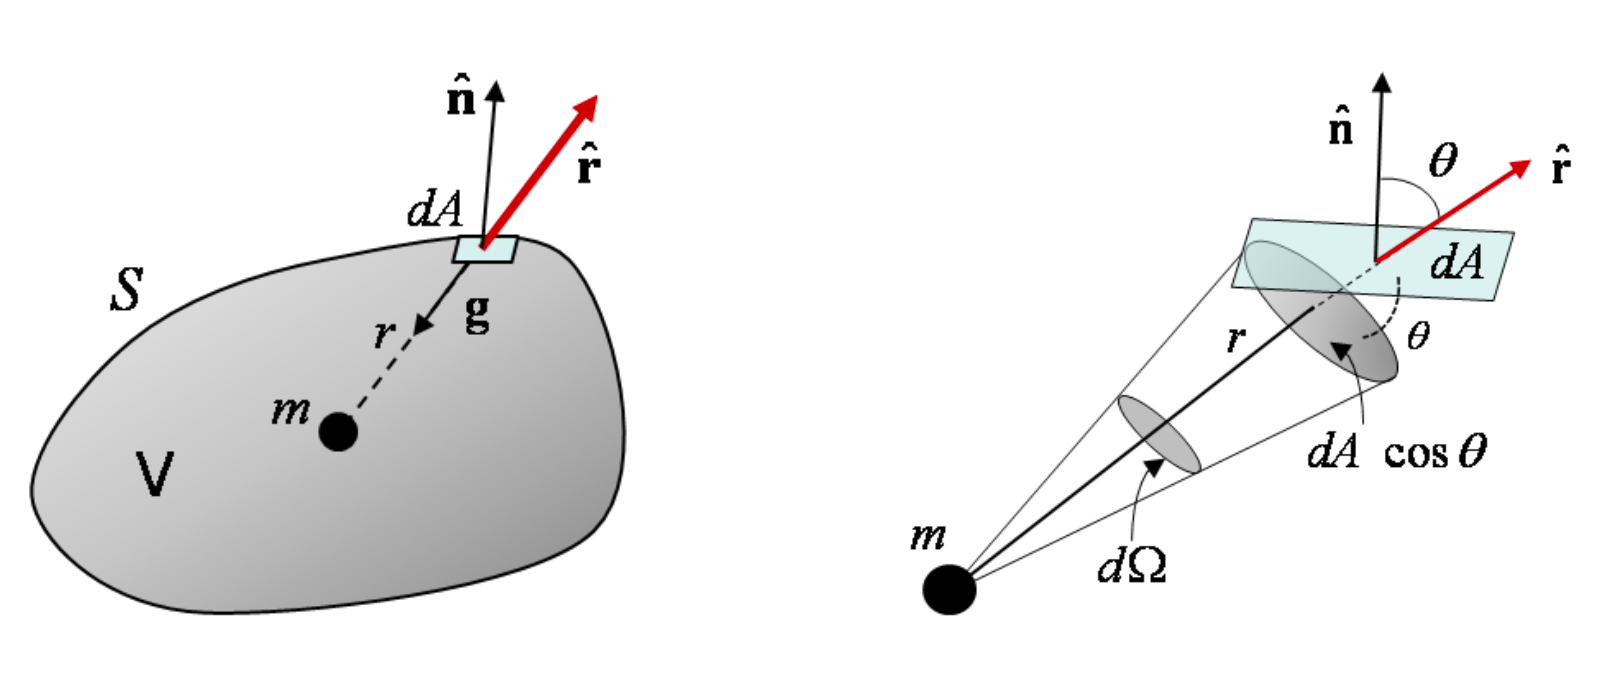
\includegraphics[width=\linewidth]{FlujoGravitacional.png}
\end{column}
\end{columns}
\begin{itemize}
\item<4-> $\oint_S d\Omega=4\pi$ ($m$ dentro de $S$) o $0$ ($m$ fuera) $\Rightarrow$ $\Phi=-4\pi Gm$ o $\Phi=0$.
\item<5-> Consecuencia exacta de $f\propto r^{-2}$: $1/r^2$ compensa el área $\propto r^2$.
\end{itemize}
\end{frame}

%==================================================================
\begin{frame}{Ley de Gauss y ecuación de Poisson}
\begin{itemize}
\item<1-> Por superposición,
\[\oint_S\mathbf g\cdot d\mathbf A=-4\pi G\,M_{\mathrm{enc}},\qquad
M_{\mathrm{enc}}=\sum_{i\,\in\,\mathcal V}m_i\ \longrightarrow\ \int_{\mathcal V}\rho\,d^3x
\]
(masas externas a $S$ no contribuyen al flujo).
\item<2-> Teorema de la divergencia:
\(\displaystyle\int_{\mathcal V}\big(\nabla\cdot\mathbf g+4\pi G\rho\big)\,d^3x=0\) \ para toda región $\mathcal V$.
\item<3-> Si el integrando es continuo y $\mathcal V$ es arbitraria:
\[\nabla\cdot\mathbf g=-4\pi G\rho \qquad\text{(Gauss, forma diferencial).}\]
\item<4-> Con $\mathbf g=-\nabla\varphi$:
\[\boxed{\nabla^2\varphi=4\pi G\rho}\quad\text{(Poisson)};\qquad \rho=0\ \Rightarrow\ \nabla^2\varphi=0\ \text{(Laplace)}.\]
\item<5-> Comprobación: masa puntual, $\rho=m\,\delta^3(\vr)$; como $\nabla^2(1/r)=-4\pi\delta^3(\vr)$, $\varphi=-Gm/r$ satisface Poisson. $\checkmark$
\end{itemize}
\end{frame}

%==================================================================
\begin{frame}{¿Por qué importa en el problema de Kepler?}
\begin{itemize}
\item<1-> Cuerpo con densidad $\rho=\rho(r)$ (simetría esférica) $\Rightarrow$ por simetría $\mathbf g=g(r)\,\ur$.
\item<2-> Ley de Gauss sobre una esfera de radio $r$:
\[4\pi r^2g(r)=-4\pi G\,M(r),\qquad M(r)=4\pi\int_0^r\rho(r')\,r'^2\,dr' ,\]
\[\mathbf g=-\frac{GM(r)}{r^2}\,\ur\ \ \xrightarrow{\ r>R\ }\ \ -\frac{GM}{r^2}\,\ur .\]
\item<3-> Fuera de un cuerpo esférico el campo es \alert{exactamente} el de una masa puntual (teorema de la cáscara de Newton): esto justifica tratar Sol y planetas como partículas.
\item<4-> Límites del modelo: achatamiento de los cuerpos, otros planetas, correcciones relativistas $\Rightarrow$ perturbaciones de $-k/r$ (precesión, sesiones siguientes).
\end{itemize}
\end{frame}

%==================================================================
\section{La ecuación de la órbita (Binet)}
\begin{frame}{Ecuación de la órbita (1/2): de $t$ a $\theta$}
\begin{itemize}
\item<1-> Objetivo: una ecuación para $r(\theta)$ eliminando $t$. \\
Supuesto: $L\neq0$ (si $L=0$ el movimiento es radial y $\theta$ no está definida).
\item<2-> Con $L>0$, $\dot\theta=L/(\mu r^2)>0$: $\theta(t)$ es monótona y sirve de parámetro,
\[\frac{d}{dt}=\dot\theta\,\frac{d}{d\theta}=\frac{L}{\mu r^2}\,\frac{d}{d\theta}.\]
\item<3-> Con $u\equiv1/r$: \ $\dfrac{du}{d\theta}=-\dfrac{1}{r^2}\dfrac{dr}{d\theta}$, \ luego
\[\dot r=\frac{L}{\mu r^2}\frac{dr}{d\theta}=-\frac{L}{\mu}\frac{du}{d\theta}.\]
\item<4-> Derivando otra vez con respecto a $t$:
\[\ddot r=\frac{L u^2}{\mu}\,\frac{d}{d\theta}\!\left(-\frac{L}{\mu}\frac{du}{d\theta}\right)
=-\frac{L^2u^2}{\mu^2}\,\frac{d^2u}{d\theta^2}.\]
\end{itemize}
\end{frame}

%==================================================================
\begin{frame}{Ecuación de la órbita (2/2): ecuación de Binet}
\begin{itemize}
\item<1-> Lado derecho: \ $\dfrac{dV}{dr}=\dfrac{dV}{du}\dfrac{du}{dr}=-u^2\dfrac{dV}{du}$.
\item<2-> Sustituyendo en $\mu\ddot r-L^2u^3/\mu=-dV/dr$:
\[-\frac{L^2}{\mu}u^2\frac{d^2u}{d\theta^2}-\frac{L^2}{\mu}u^3=u^2\frac{dV}{du}.\]
\item<3-> Dividiendo entre $-u^2$:
\[\boxed{\ \frac{L^2}{\mu}\left(\frac{d^2u}{d\theta^2}+u\right)=-\frac{dV}{du}\ }\qquad\text{(ecuación de Binet)}\]
\item<4-> En términos de la fuerza, $f=-dV/dr$: \quad
$\dfrac{d^2u}{d\theta^2}+u=-\dfrac{\mu}{L^2u^2}\,f\!\left(\dfrac1u\right)$.
\item<5-> Dimensiones: $[L^2u/\mu]=[dV/du]=\mathrm{J\,m}$. $\checkmark$
\item<6-> Dos usos: \alert{directo} (dado $V$, hallar $r(\theta)$) e \alert{inverso} (dada $r(\theta)$, hallar $f(r)$).
\end{itemize}
\end{frame}

%==================================================================
\begin{frame}{Problema inverso: la cónica kepleriana}
\begin{itemize}
\item<1-> Órbita dada: $\dfrac{q}{r}=1+e\cos\theta$, \ es decir \ $u(\theta)=\dfrac1q\,(1+e\cos\theta)$.
\item<2-> $\dfrac{d^2u}{d\theta^2}=-\dfrac{e}{q}\cos\theta \ \Rightarrow\ \dfrac{d^2u}{d\theta^2}+u=\dfrac1q$ \ (independiente de $\theta$ y de $e$).
\item<3-> Binet en forma de fuerza:
\[ f(r)=-\frac{L^2u^2}{\mu}\left(\frac{d^2u}{d\theta^2}+u\right)=-\frac{L^2}{\mu q}\,\frac{1}{r^2}. \]
\item<4-> Una cónica con el centro de fuerza en el foco exige una fuerza atractiva $\propto r^{-2}$, con $k=L^2/(\mu q)$.
\item<5-> Para pensar: la misma elipse con el centro de fuerza en su \emph{centro geométrico} exige otra ley de fuerza. ¿Cuál?
\item<6-> Ejercicio (notas del curso, Sec.~3.3): la espiral $r=r_0e^{-a\theta}$.
\end{itemize}
% Nota instructor: centro geométrico -> f = -k r (oscilador isótropo);
% espiral -> V = -k/r^2 con k = L^2(a^2+1)/(2 mu), cae al centro.
\end{frame}

%==================================================================
\section{Solución del problema de Kepler}
\begin{frame}{Problema directo: la órbita kepleriana}
\begin{itemize}
\item<1-> $V=-k/r=-ku$, \ $k=Gm_1m_2>0$ $\Rightarrow$ $-dV/du=k$. Binet:
\[\frac{d^2u}{d\theta^2}+u=\frac{\mu k}{L^2}\equiv\frac1q .\]
\item<2-> EDO lineal de segundo orden, inhomogénea, con coeficientes constantes: un oscilador armónico en $\theta$ con forzamiento constante.
\item<3-> Homogénea: $u_h=A\cos(\theta-\theta_0)$; \ particular: $u_p=1/q$.
\item<4-> Solución general:
\[\frac1r=\frac1q\big[1+e\cos(\theta-\theta_0)\big],\qquad q=\frac{L^2}{\mu k},\qquad e\equiv Aq=\frac{AL^2}{\mu k}.\]
\item<5-> Sin pérdida de generalidad $A\ge0$ (el signo se absorbe en $\theta_0$), luego $e\ge0$. $\theta_0$ es la dirección del pericentro; tomamos $\theta_0=0$ orientando el eje polar hacia él.
\item<6-> $u(\theta)$ tiene período $2\pi$: la órbita acotada se cierra y el pericentro \alert{no precesa}.
\end{itemize}
\end{frame}

%==================================================================
\begin{frame}{Excentricidad y energía}
\begin{itemize}
\item<1-> ¿Qué fija $e$? Evaluamos $E$ en el pericentro, donde $\dot r=0$ y $u_{\max}=(1+e)/q$:
\[E=\Vef(r_{\min})=\frac{L^2}{2\mu}\,u_{\max}^2-k\,u_{\max}.\]
\item<2-> Con $q=L^2/(\mu k)$:
\[E=\frac{\mu k^2}{L^2}\left[\frac{(1+e)^2}{2}-(1+e)\right]=\frac{\mu k^2}{2L^2}\,\big(e^2-1\big).\]
\item<3-> Por tanto
\[\boxed{\ e=\sqrt{1+\frac{2EL^2}{\mu k^2}}\ }\]
La órbita queda fijada por $(E,L,\theta_0)$; la cuarta constante, $t_0$, fija el paso por el pericentro.
\item<4-> Chequeos: $2EL^2/(\mu k^2)$ es adimensional; $e$ real $\Leftrightarrow E\ge-\mu k^2/(2L^2)=\min\Vef$. $\checkmark$
% Alternativa para mencionar oralmente: cuadratura de theta(u) (notas, Ecs. 3.109-3.114).
\end{itemize}
\end{frame}

%==================================================================
\begin{frame}{Geometría de la cónica}
\begin{columns}[T]
\begin{column}{0.60\textwidth}
\begin{itemize}
\item<1-> $q/r=1+e\cos\theta$, \ foco en el origen.
\item<2-> $q=r(\pi/2)=L^2/(\mu k)$: \alert{semilado recto} (\emph{semi-latus rectum}; el lado recto mide $2q$).
\item<3-> Pericentro: $r_{\min}=r(0)=\dfrac{q}{1+e}$.
\item<4-> Si $e<1$: $r_{\max}=r(\pi)=\dfrac{q}{1-e}$ y
\[a=\frac{r_{\min}+r_{\max}}{2}=\frac{q}{1-e^2}=\frac{k}{2|E|},\]
que depende solo de $E$.
\item<5-> Si $e\ge1$: $r\to\infty$ cuando $\cos\theta\to-1/e$; la órbita solo ocupa $|\theta|<\arccos(-1/e)$.
\end{itemize}
\end{column}
\begin{column}{0.38\textwidth}
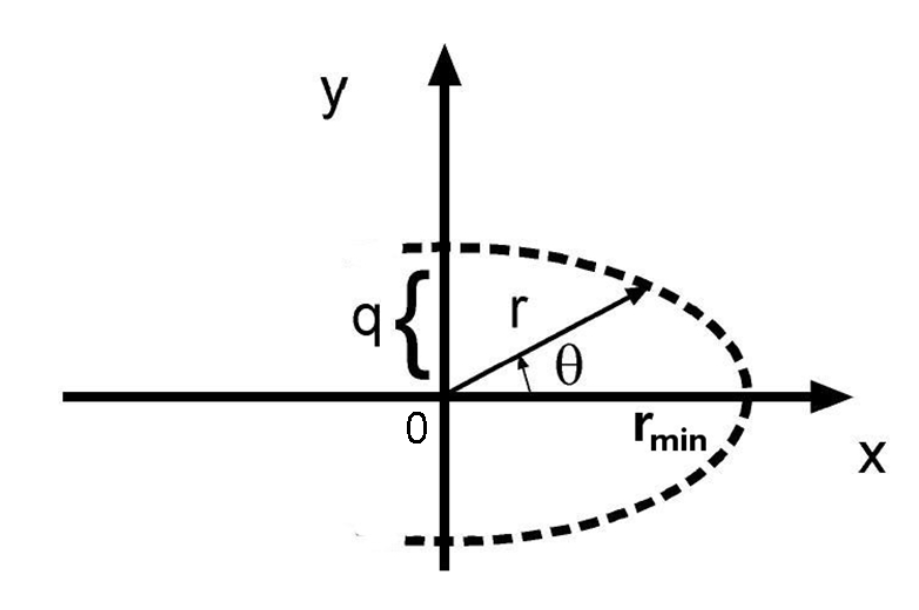
\includegraphics[width=\linewidth]{Conica.png}
\end{column}
\end{columns}
\end{frame}

%==================================================================
\section{Clasificación de órbitas}
\begin{frame}{Potencial efectivo del problema de Kepler}
\begin{columns}[T]
\begin{column}{0.58\textwidth}
\begin{itemize}
\item<1-> Movimiento radial en
\[\Vef(r)=-\frac kr+\frac{L^2}{2\mu r^2}.\]
\item<2-> Mínimo, $\Vef'(r_0)=0$:
\[r_0=\frac{L^2}{\mu k}=q,\qquad \Vef(r_0)=-\frac{\mu k^2}{2L^2}.\]
\item<3-> Puntos de retorno: raíces de $E=\Vef(r)$, i.e.\ $Er^2+kr-\dfrac{L^2}{2\mu}=0$; coinciden con $q/(1\pm e)$.
\item<4-> $E<0$: movimiento radial acotado; $E\ge0$: no acotado.
\end{itemize}
\end{column}
\begin{column}{0.40\textwidth}
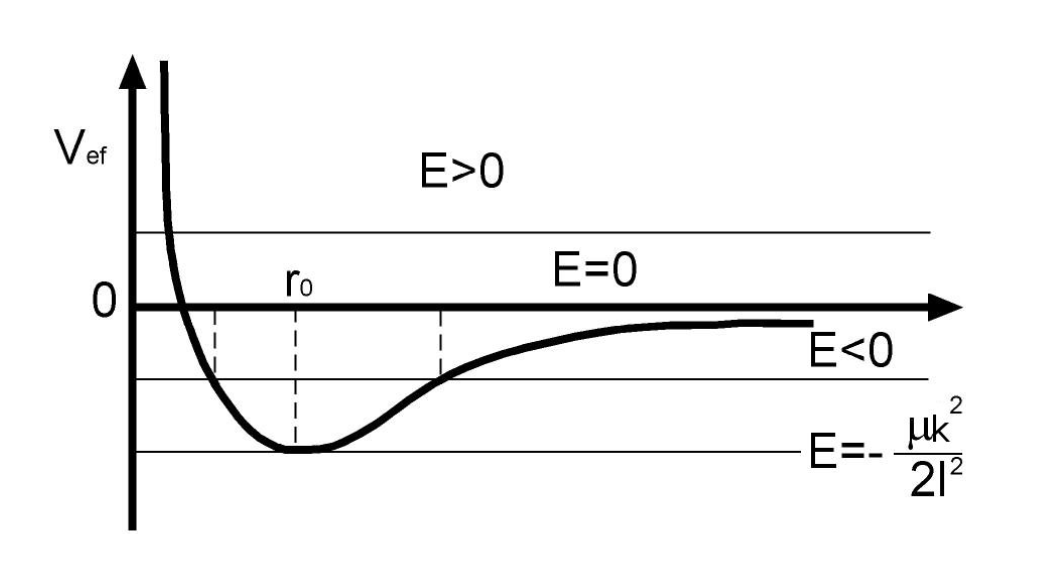
\includegraphics[width=\linewidth]{KeplerEfectivo.png}
\end{column}
\end{columns}
\end{frame}

%==================================================================
\begin{frame}{Órbitas, excentricidades y energías}
\begin{center}
\small\renewcommand{\arraystretch}{1.2}
\begin{tabular}{@{}cccc@{}}
\toprule
$e$ & $E$ & Órbita & Mov.\ radial \\
\midrule
$0$ & $-\mu k^2/2L^2$ & circunferencia ($r=q$) & $r$ constante \\
$(0,1)$ & $(-\mu k^2/2L^2,\,0)$ & elipse & $r_{\min}\le r\le r_{\max}$ \\
$1$ & $0$ & parábola & no acotado \\
$>1$ & $>0$ & hipérbola & no acotado \\
\bottomrule
\end{tabular}
\end{center}
\begin{columns}[c]
\begin{column}{0.40\textwidth}
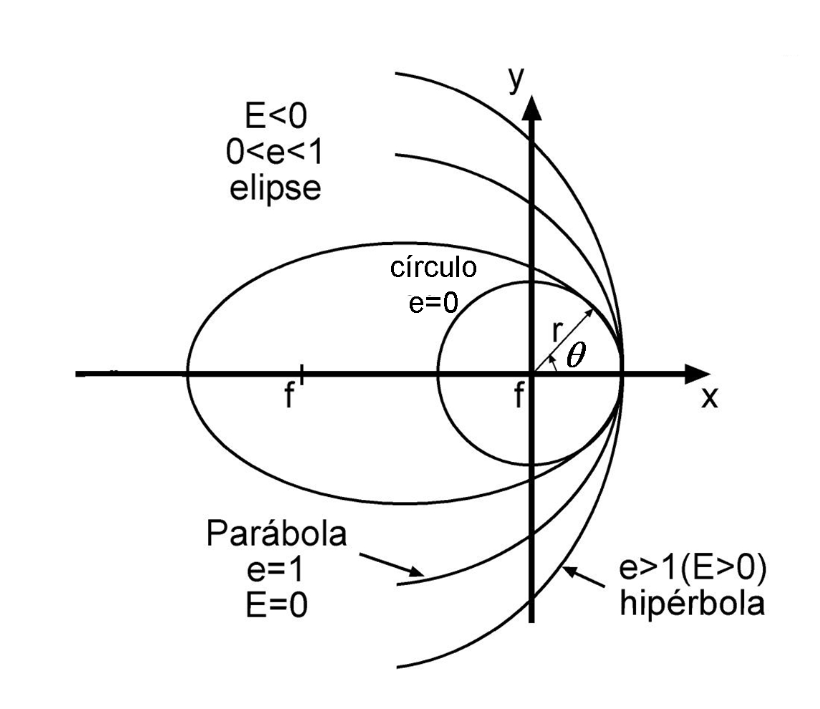
\includegraphics[width=\linewidth]{OrbitaKepler.png}
\end{column}
\begin{column}{0.53\textwidth}
\begin{itemize}
\item<2-> El \alert{signo de $E$} decide si la órbita es cerrada o abierta.
\item<3-> La circunferencia exige además $E=\min\Vef$, que depende de $L$: la clasificación completa requiere $(E,L)$.
\end{itemize}
\end{column}
\end{columns}
\end{frame}

%==================================================================
\section{Verificación, IA y cómputo}
\begin{frame}{Verificaciones conceptuales}
\begin{enumerate}
\item<1-> Con $E<0$ fija, se duplica $L$. ¿Cambia $a$? ¿Cambia $e$? Justifique sin calcular la órbita.
\item<2-> ¿Por qué el pericentro es un punto conveniente para evaluar $E$? ¿Serviría $\theta=\pi/2$?
\item<3-> Un estudiante afirma: ``si $E<0$ la órbita es una elipse, luego $e$ depende solo de $E$''. ¿Qué es incorrecto?
\item<4-> ¿Qué ocurre con la ecuación de Binet cuando $L\to0$? ¿Qué describe el límite $e\to1$ con $E<0$ fija?
\item<5-> ¿Qué propiedad de $u''+u=\text{cte}$ garantiza que la órbita se cierre? ¿Seguiría cerrándose con $V=-k/r+\epsilon/r^2$?
\end{enumerate}
% Notas instructor:
% 1) a = k/2|E| no cambia; e = sqrt(1-L^2/(mu k a)) disminuye (L^2 -> 4L^2).
% 2) Allí rdot = 0 y E = Veff; en theta = pi/2 también sirve pero exige rdot != 0.
% 3) e depende de E y L (ver tabla).
% 4) Binet deja de valer (theta no es parámetro); órbita degenerada: segmento radial.
% 5) Período 2*pi en theta. Con eps/r^2: u'' + (1 + 2 mu eps/L^2) u = cte -> precesión.
\end{frame}

%==================================================================
\begin{frame}{Actividad con IA: auditar una derivación}
\small
\textbf{Política:} uso de IA \alert{requerido} para análisis crítico; entrega individual.
\begin{enumerate}
\item<1-> Pida a un asistente de IA: \emph{``Deriva la ecuación de Binet para un potencial central $V(r)$ y resuélvela para $V=-k/r$, obteniendo $e(E,L)$''}.
\item<2-> Audite la respuesta con tres pruebas independientes:
  (a) dimensiones de cada término; (b) signo: ¿la fuerza que implica es atractiva?;
  (c) límite circular: $e=0 \Leftrightarrow E=\min\Vef$.
\item<3-> Variante controlada (entregada por el profesor): una derivación con
  $dV/dr=+u^2\,dV/du$. Localice el error y explique qué consecuencia física absurda produce para $E<0$.
\item<4-> Documente: prompts usados; fragmento relevante de la respuesta; qué aceptó, rechazó o corrigió; cómo lo verificó; su derivación final; errores o ``alucinaciones'' detectados.
\end{enumerate}
% Nota instructor: con el signo errado se obtiene u'' + u = -1/q, es decir
% 1/r = (e cos theta - 1)/q: no existe órbita acotada y la trayectoria rodea
% el foco exterior, como en una fuerza repulsiva.
\end{frame}

%==================================================================
\begin{frame}{Extensión computacional (Python)}
\begin{itemize}
\item<1-> Deduzca primero las ecuaciones en variables cartesianas: $\mu\ddot{\vr}=-k\,\vr/r^3$. Unidades adimensionales $\mu=k=1$.
\item<2-> Integre una órbita con $e=0.6$ y compare $r(\theta)$ numérico con $q/(1+e\cos\theta)$.
\item<3-> Monitoree $E$, $L$ y la dirección del pericentro durante 100 períodos con
  \begin{itemize}
  \item RK4 de paso fijo, y
  \item Verlet (simpléctico) con el mismo paso.
  \end{itemize}
\item<4-> Ambos métodos muestran una \alert{precesión espuria} del pericentro. Mida cómo escala con el paso $h$ y compárela con la deriva de $E$. ¿Cómo sabe que no es un efecto físico?
\item<5-> Entregable: código documentado y reproducible, gráficas de $\Delta E/E$ y $\Delta L/L$ contra $t$, e interpretación.
\end{itemize}
% Nota instructor: RK4 -> deriva secular de E y L (la órbita decae); Verlet ->
% L conservado a redondeo (fuerza central), error en E acotado y oscilante, pero
% precesión O(h^2) (conserva un Hamiltoniano "sombra" que no es el de Kepler).
% Criterio de artefacto: el efecto desaparece al reducir h con el orden esperado,
% mientras que la solución exacta tiene A (vector LRL) constante.
\end{frame}

%==================================================================
\begin{frame}{Resumen y conexión con lo que sigue}
\begin{itemize}
\item<1-> Binet: $\dfrac{L^2}{\mu}\big(u''+u\big)=-\dfrac{dV}{du}$, válida para todo potencial central con $L\neq0$.
\item<2-> Kepler: $\dfrac{q}{r}=1+e\cos(\theta-\theta_0)$, \ $q=\dfrac{L^2}{\mu k}$, \ $e=\sqrt{1+\dfrac{2EL^2}{\mu k^2}}$, \ $a=\dfrac{k}{2|E|}$.
\item<3-> Supuestos: dos cuerpos puntuales o esféricos, gravitación newtoniana, sin perturbaciones.
\item<4-> Próximas sesiones:
  \begin{itemize}
  \item leyes de Kepler y dependencia temporal (ecuación de Kepler);
  \item estabilidad de órbitas circulares y precesión;
  \item vector de Laplace--Runge--Lenz: la simetría ``oculta'' que explica por qué $\theta_0$ es constante;
  \item dispersión: la rama hiperbólica ($E>0$).
  \end{itemize}
\end{itemize}
\end{frame}

\end{document}
